\documentclass[a4paper, 11pt, notitlepage]{article}
\addtolength{\hoffset}{-1cm}
\addtolength{\textwidth}{2cm}
\usepackage[utf8]{inputenc}
\usepackage[frenchb]{babel}
\usepackage[T1]{fontenc}

\usepackage{listings}
\usepackage{graphicx}

\ProvidesPackage{mips}
\usepackage{color}
\RequirePackage{listings}
 
\lstdefinelanguage[mips]{Assembler}{%
  % so listings can detect directives and register names
  alsoletter={.\$},
  % strings, characters, and comments
  morestring=[b]",
  morestring=[b]',
  morecomment=[l]\#,
  % instructions
  morekeywords={[1]abs,abs.d,abs.s,add,add.d,add.s,addi,addiu,addu,%
    and,andi,b,bc1f,bc1t,beq,beqz,bge,bgeu,bgez,bgezal,bgt,bgtu,%
    bgtz,ble,bleu,blez,blt,bltu,bltz,bltzal,bne,bnez,break,c.eq.d,%
    c.eq.s,c.le.d,c.le.s,c.lt.d,c.lt.s,ceil.w.d,ceil.w.s,clo,clz,%
    cvt.d.s,cvt.d.w,cvt.s.d,cvt.s.w,cvt.w.d,cvt.w.s,div,div.d,div.s,%
    divu,eret,floor.w.d,floor.w.s,j,jal,jalr,jr,l.d,l.s,la,lb,lbu,%
    ld,ldc1,lh,lhu,li,ll,lui,lw,lwc1,lwl,lwr,madd,maddu,mfc0,mfc1,%
    mfc1.d,mfhi,mflo,mov.d,mov.s,move,movf,movf.d,movf.s,movn,movn.d,%
    movn.s,movt,movt.d,movt.s,movz,movz.d,movz.s,msub,msubu,mtc0,mtc1,%
    mtc1.d,mthi,mtlo,mul,mul.d,mul.s,mulo,mulou,mult,multu,mulu,neg,%
    neg.d,neg.s,negu,nop,nor,not,or,ori,rem,remu,rol,ror,round.w.d,%
    round.w.s,s.d,s.s,sb,sc,sd,sdc1,seq,sge,sgeu,sgt,sgtu,sh,sle,%
    sleu,sll,sllv,slt,slti,sltiu,sltu,sne,sqrt.d,sqrt.s,sra,srav,srl,%
    srlv,sub,sub.d,sub.s,subi,subiu,subu,sw,swc1,swl,swr,syscall,teq,%
    teqi,tge,tgei,tgeiu,tgeu,tlt,tlti,tltiu,tltu,tne,tnei,trunc.w.d,%
    trunc.w.s,ulh,ulhu,ulw,ush,usw,xor,xori},
  % assembler directives
  morekeywords={[2].align,.ascii,.asciiz,.byte,.data,.double,.extern,%
    .float,.globl,.half,.kdata,.ktext,.set,.space,.text,.word},
  % register names
  morekeywords={[3]\$0,\$1,\$2,\$3,\$4,\$5,\$6,\$7,\$8,\$9,\$10,\$11,%
    \$12,\$13,\$14,\$15,\$16,\$17,\$18,\$19,\$20,\$21,\$22,\$23,\$24,%
    \$25,\$26,\$27,\$28,\$29,\$30,\$31,%
    \$zero,\$at,\$v0,\$v1,\$a0,\$a1,\$a2,\$a3,\$t0,\$t1,\$t2,\$t3,\$t4,
    \$t5,\$t6,\$t7,\$s0,\$s1,\$s2,\$s3,\$s4,\$s5,\$s6,\$s7,\$t8,\$t9,%
    \$k0,\$k1,\$gp,\$sp,\$fp,\$ra},
}[strings,comments,keywords]


\lstnewenvironment{mips}
                  {\lstset{
                      language=[mips]Assembler,
                      breaklines=true,
                      showstringspaces=false,
                      commentstyle=\color{red},
                      stringstyle=\color{darkgray},
                      identifierstyle=\ttfamily,
                      keywordstyle=\color{blue},
                      basicstyle=\footnotesize,
                      escapeinside={/*}{*/},
                      %xleftmargin=0.08\textwidth
                    }
                  }
                  {}



\title{
  Projet de Compilation Avancée
}
\author{
  Béatrice Carré \and Stéphane Ferreira \and Marwan Ghanem 
}

\begin{document}

\maketitle

\

\section*{Introduction}
Ce projet a pour objectif la prise en main des méthodes d'optimisation
de code assembleur et l'application des concepts
étudiés en cours. Pour ce faire, nous avons dû étudier les dépendances entre blocs, les dépendances entre els instruction, les graphes de flot de contrôle, les graphes de flot de données et les chemins critiques.

Après cela, nous avons pu atteindre  la phase de réordonnancement du code, qui est 
une véritable technique d'optimisation. Nous détaillons dans ce rapport toutes les fonctionnalités implémentées du projet accompagnés d'un exemple d'exécution. 
\

\

\section{Reconnaissance des fonctions}

Pour cette phase, il est nécessaire de parcourir chaque ligne du code assembleur et identifier les
fonctions. Elle sont délimitées par les deux directive \emph{.ent} et
\emph{.end}. Nous avons donc simplement créé une nouvelle fonction (la
classe \emph{Function}) à chaque directive \emph{.ent} rencontrée, et indiqué sa
fin à la directive \emph{.end} suivante. 

La fonction implémentant ceci est \verb comput_function  dans la classe \emph{Program}. 

\section{Reconnaissance des blocs de base}

Il faut maintenant identifier les blocs de base pour chaque fonction. On
parcourt les lignes de la fonction en déterminant le début et
fin de bloc selon les règles suivantes : 
\begin{itemize}
\item Un label correspond à un début de bloc, cela veut aussi dire que la ligne
  précédente est la fin d'un bloc. 
\item Une instruction de type branchement correspond à un saut et indique donc la
  fin d'un bloc mais il faut prendre en compte le delayed slot qui
  fait partie du bloc. La fin de celui-ci est donc l'instruction suivante. 
\end{itemize}

Cela correspond à la fonction \verb comput_basic_block de la classe \emph{Function}.

\section{Dépendances entre les blocs de base}

On s'intéresse maintenant aux dépendances entre blocs de base.
Il faut ici déterminer les blocs successeurs et prédécesseurs pour
chaque bloc.
Les blocs prédécesseurs et successeurs sont déterminés ainsi : 
\begin{itemize}
\item Si l'instruction correspond à un nop (``add \$0, \$0, \$0''), 
  alors on traite l'instruction précédente, qui correspond à un branchement :
  \begin{itemize}
  \item Si cette instruction est un appel de fonction (``jal label''), alors 
    le bloc successeur est celui auquel correspond le label
  \item Si c'est autre saut inconditionnel, alors le successeur est le bloc de base correspondant au label.
  \item Sinon, c'est un branchement conditionnel, alors la
  cible du saut (le bloc qui commence par le label visé dans le saut)
  et le bloc suivant, s'il y en a un, sont ses successeurs
  \end{itemize}
\item Sinon, le successeur est simplement le bloc suivant dans le code.

\end{itemize}

Voir \verb |comput_succ_pred_BB| dans la classe \emph{Function}.

\section{Construction des graphes de flot de contrôle}

Le code pour la construction de ces graphes étant donné,
le seul travail à faire ici a été, pour chaque fonction du
programme, de créer un nouveau CFG en indiquant le premier 
bloc de base de la fonction et son nombre de bloc de base. 
En annexe vous pouvez voir le CFG de la fonction \emph{MAT\_MUL} du
fichier \emph{test\_asm32.s}.

Voir \verb |comput_cfg| de la classe \emph{Program}.

\section{Dépendances entre les instructions}

On s'intéresse ici aux dépendances entre instructions appartenant à un
même bloc de base. 
Pour cela, pour chaque instruction étudiée en partant de la dernière, on la compare avec toutes celles au dessus d'elle selon les règles suivantes :
\begin{itemize}
  \item S'il y a une dépendance de type RAW avec le premier opérateur
    lu (RAW1) et qu'il n'y en a pas encore, alors on l'ajoute.
  \item S'il y a une dépendance de type RAW avec le deuxième opérateur lu (RAW2) et qu'il n'y en a pas encore, alors on l'ajoute.
  \item S'il y a une dépendance WAR, et qu'il n'y a pas encore eu de dépendance WAW, on l'ajoute.
  \item S'il y a une dépendance WAW, et qu'il n'y en a pas encore eu, on indique qu'on en a rencontré une, et on l'ajoute s'il n'y a pas encore eu de dépendance WAR.
  \item Si on a déjà rencontré un dépendance de type RAW1, RAW2 et WAW, alors il n'y a plus de dépendance à trouver pour cette instruction étudiée, on passe à la suivante.
\end{itemize}
Ce traitement est fait
dans la fonction \verb |comput_pred_succ_dep| de la classe
\emph{Basic\_block}. 

\section{Construction du graphe de flot de données}

A partir des dépendances entre les instructions, la construction
du graphe de flot de données (DFG) d'un bloc suit simplement ce qui a été vu en cours. 
On parcourt une première fois les instructions pour créer les noeuds (la classe Node\_dfg) et pour récupérer le noeud correspondant au saut de fin de bloc s'il y en a un. On fait ensuite
une deuxième itération pour effectuer sur chaque noeud le traitement suivant : 
\begin{itemize}
\item Si le noeud n'a pas de prédécesseur et que ce n'est pas un branchement, alors on l'ajoute à la liste des racines \emph{\_roots} du DFG. 
\item Si le noeud représente un saut, alors il correspond au saut de fin de
  bloc et on ajoute le noeud suivant (qui correspond à l'instruction nop) à la liste \emph{\_delayed\_slot} du DFG.
\item Pour chaque successeur de l'instruction, on va chercher le noeud le
  représentant, et on ajoute au DFG un nouvel arc avec la
  dépendance concernée par les deux noeuds et le délai qui correspond. 
\end{itemize}
Le résultat de cette fonction sur l'exemple \emph{test\_asm32.s} est en annexe.

Ce comportement est implémenté dans le constructeur de la classe Dfg.

\section{Calcul du chemin critique}

Le calcul du chemin critique se fait avec l'algorithme étudié en cours. La
méthode \verb|get_inverse_topoligic_order| a été ajoutée pour calculer
l'ordre topologique inverse (les noeuds successeurs d'abord) nécessaire à la construction du chemin critique. 

L'algorithme est le suivant : à partir d'une liste temporaire des noeuds sans
successeurs. Pour chaque noeud dans la liste temporaire (à partir du premier), on
l'ajoute à la fin de la liste finale, puis on ajoute ses prédécesseurs à la fin
de la liste temporaire. On itère ce processus jusqu'à ce que la liste
temporaire soit vide.

Après, le calcul du chemin critique se fait comme l'algorithme décrit dans le cours :
On initialise tous les noeuds à 0, puis on parcourt chaque noeud dans l'ordre topologique inverse : si c'est une feuille, alors son poids est égale à sont temps d'exécution, sinon son poids est égal au max, entre tous ses successeurs, entre le délai avec celui-ci ajouté au poids de ce successeur.

Une fois ce calcul fait, le chemin critique est le poids max entre tous les noeuds sans prédécesseur.

Cet algorithme est implémenté dans les méthodes \verb|comput_critical_path| et 

\noindent
\verb|get_critical_path| de la class \emph{Dfg}.

\newpage
\section{Réordonnancement avec l'algorithme de liste}

Le réordonnancement s'effectue selon l'algorithme d'ordonnancement par liste vu en
cours, nous ne nous attarderons donc pas sur cet l'algorithme lui-même. 
Pour le traitement, on s'appuie sur la liste
\emph{\_inst\_ready} contenant les instructions prêtes à être
traitées. Au début, cette liste doit contenir les racines du DFG. Tant qu'il
reste des élements à cette liste, il faut continuer le traitement qui détermine
 laquelle de ces instructions il faut
choisir. Pour cela, on trie la liste (en s'aidant de la
fonction \emph{sort} des listes) en ordre croissant des priorités, c'est à
dire que l'on trie d'abord selon les index, et finir par trier selon
les poids. La seule priorité légèrement différente est celle qui vérifie
qu'on n'engendre pas de cycles de gel. Pour cela, il faut vérifier
que pour chaque instruction réordonnancée, le délai avec celle
en cours de traitement n'excède pas la différence d'index entre
celles-ci. 

Voir la fonction \verb |scheduling| de la classe \emph{Dfg}.

\section{Bonus : Renommage de registres}
Pour faire cette phase, nous avons dû créer une fonction dans la classe \emph{Instruction} (\verb |is_WR|), pour savoir si l'instruction est de type écriture, c'est à dire si elle écrit dans un registre.
Ainsi qu'une fonction dans la classe \emph{Basic\_Block} (\verb |contains|) pour savoir si le registre est dans la liste des registres non vivants.

Ici, on suppose que le nombre de registres disponibles pour le renommage n'est pas borné.
L'algo de renommage de registre est le suivant :

On parcourt chaque instruction du bloc, si on fait une écriture dans un registre, et si le registre qui est écrit fait partie de la liste des registres non vivants :
on stocke le numéro du registre, on définit un nouveau registre libre (à partir de \$32), et et pour chaques instruction, on renomme tous les registres du même nom que celui stocké jusqu'à retomber à nouveau sur une écriture dans un registre.
\newpage
\section*{Annexe}

Voici le résultat des DFG, CFG et le code optimisé de notre programme sur le fichier de test 

\begin{figure}[!h]
  \centering
  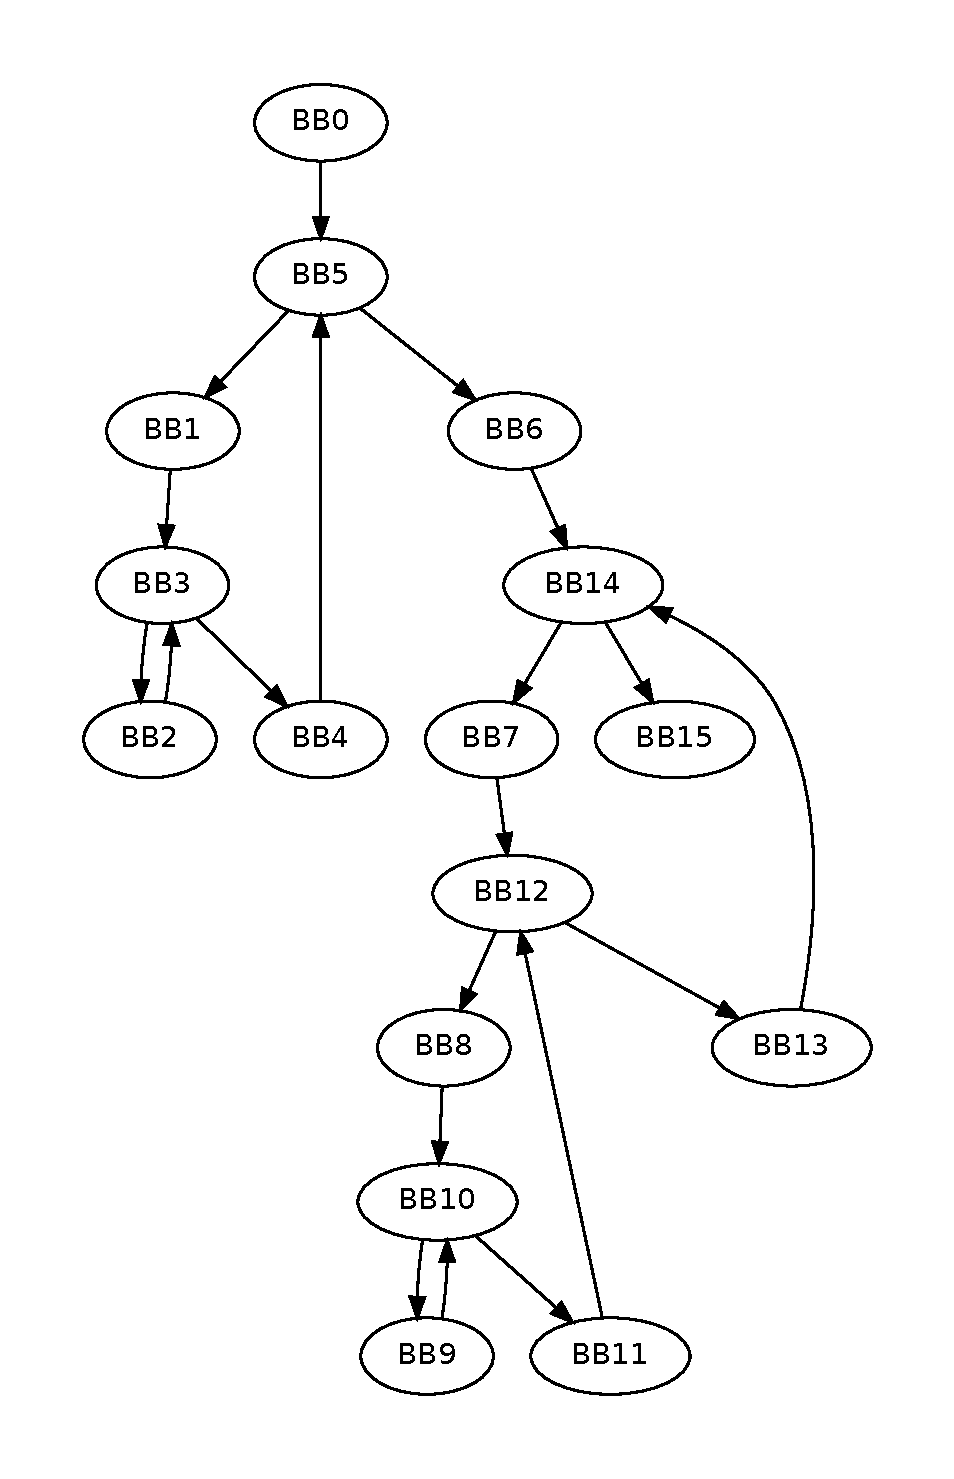
\includegraphics[scale=0.70]{mat_mul_cfg.pdf}
  \caption{CFG de la fonction MAT\_MUL du fichier d'exemple \emph{test\_asm32.s}}
\end{figure}
\newpage
\begin{figure}[!h]
  \centering
  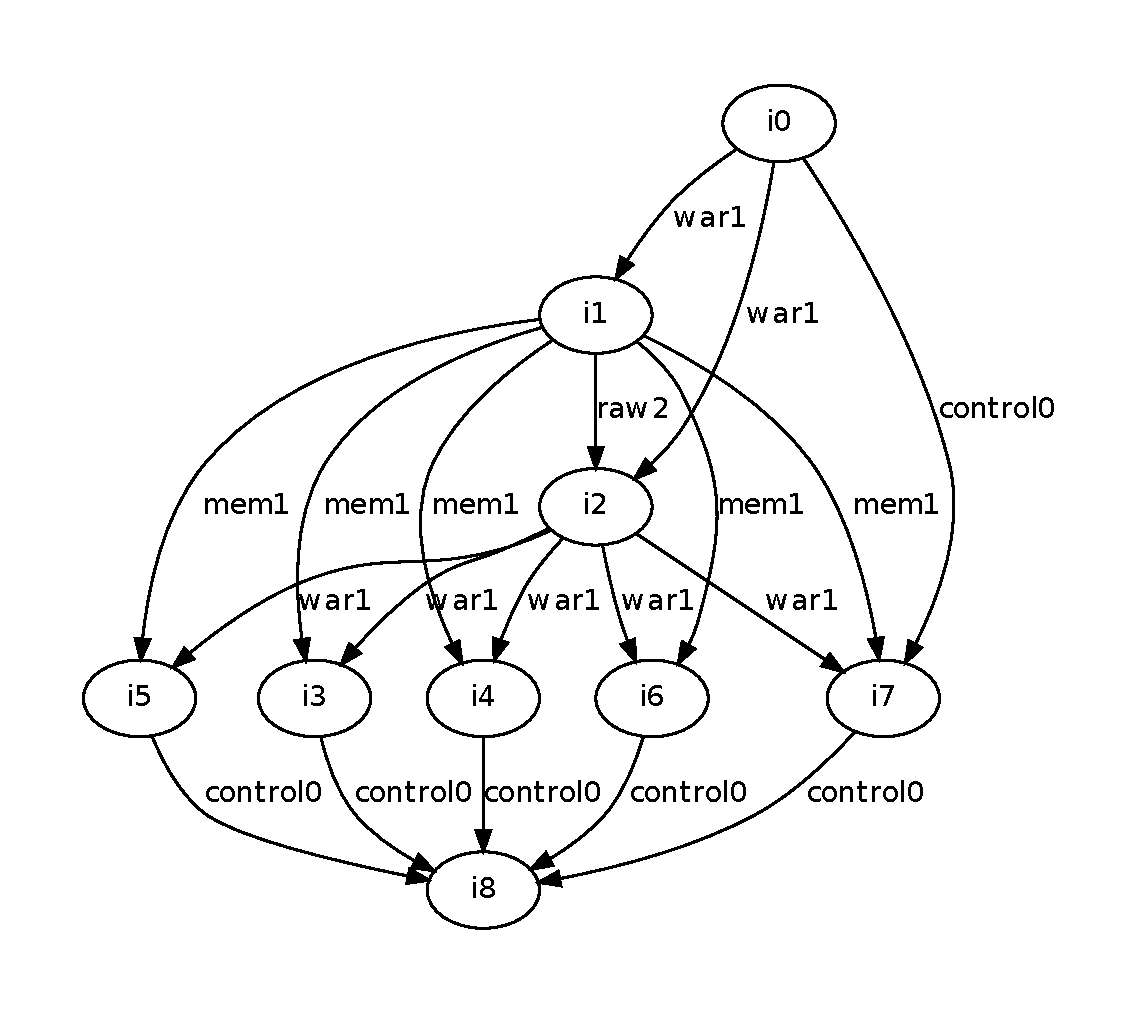
\includegraphics[scale=0.80]{sum_dfg.pdf}
  \caption{DFG de la fonction SUM du fichier d'exemple \emph{test\_asm32.s}}
\end{figure}


\newpage
Code de la fonction SUM avant et après optimisation :

\
\newline
Avant :SUM
temps critique : 5

\begin{mips}
i0 addiu $29,$29,65520
i1 sw $30,12($29)
i2 or $30,$29,$0
i3 sw $4,16($30)
i4 sw $5,20($30)
i5 sw $6,24($30)
i6 sw $7,28($30)
i7 sw $0,0($30)
i8 j $l2
i9 add $0,$0,$0
\end{mips}

Apres : SUM

\begin{mips}
i0: addiu $29,$29,65520
i1: sw $30,12($29)
i2: or $30,$29,$0
i7: sw $0,0($30)
i8: j $l2
i3: sw $4,16($30)
i4: sw $5,20($30)
i5: sw $6,24($30)
i6: sw $7,28($30)
\end{mips}

\end{document}
